\documentclass[preprint2]{aastex}
\usepackage{color}
\usepackage{natbib}
\bibliographystyle{apj}

\newcommand{\vdag}{(v)^\dagger}
\newcommand{\myemail}{eogorma@tcd.ie}

\shorttitle{The CO Shells of Betelgeuse}
\shortauthors{O'Gorman et al.}

\begin{document}

\title{CARMA CO(J=2-1) Observations of the Circumstellar \\ Envelope of Betelgeuse}

\author{Eamon O'Gorman and Graham M. Harper}
\affil{School of Physics, Trinity College Dublin, Dublin 2, Ireland}
\email{eogorma@tcd.ie}
\email{graham.harper@tcd.ie}

\author{Joanna M. Brown}
\affil{Harvard-Smithsonian Center for Astrophysics, 60 Garden Street, \\ MS-78, Cambridge, MA 02138, USA}
\email{joannabrown@cfa.harvard.edu}

\author{Seth Redfield}
\affil{Department of Astronomy, Van Vleck Observatory, Wesleyan University, \\ Middletown, CT 06459, USA}
\email{sredfield@wesleyan.edu}

\and

\author{Alexander Brown}
\affil{Center for Astrophysics and Space Astronomy, University of Colorado, \\ 389 UCB, Boulder, CO 80309, USA}
\email{alexander.brown@colorado.edu}

\begin{abstract}
We report the first radio interferometric observations of the 1.3 mm emission line of $\rm{{}^{12}}$C$\rm{{}^{16}}O$ in the circumstellar envelope of the M supergiant $\alpha$ Ori.  Observations are made with the Combined Array for Research in Millimeter-wave Astronomy (CARMA) interferometer in the C, D, and E antenna configurations. We obtain excellent  uv-coverage (6 - 27 k$\lambda$) by combining data from all three configurations allowing us to trace spatial scales from $0.9\arcsec$ to $3.9\arcsec$. The high spatial resolution C configuration map shows that the inner S1 shell has asymmetric outflow velocities of -10 km s${}^{-1}$ and +11 km s${}^{-1}$  with respect to the stellar rest frame. We find little evidence  for the outer S2 shell in this configuration and assume that the majority of this emission has been resolved out by the array. The S2 shell appears as an extra blueshifted emission component in the D and E configuration maps between -10 km s${}^{-1}$  and -17 km s${}^{-1}$ and we detect it between +11 km s${}^{-1}$ and + 14 km s${}^{-1}$ in the redshifted component of the line. A discrete off-source emission feature is detected at 5$\arcsec$ S-W of  $\alpha$ Ori in all D configuration maps. We image both shells in the combined map (all configurations) and see the formation of the classical ring structure for the S2 shell as we sample the line across velocities. We assign an outer radius of 6$\arcsec$ to S1 and believe that S2 extends beyond CARMA's field of view (32$\arcsec$ at 1.3 mm) out to a radius of 17$\arcsec$. 
\end{abstract}

\keywords{circumstellar matter --- Stars: individual: ($\rm{\alpha}$ Ori) --- Stars: late-type --- Stars: massive --- supergiants --- Radio lines: stars}

\section{INTRODUCTION}

Graham?

\section{OBSERVATIONS AND DATA REDUCTION}

The data were acquired with the 15 element Combined Array for Research in Millimeter-wave Astronomy (CARMA) interferometer \citep{2004ASPC..314..768S} which is located at Cedar Flat in eastern California. The array consists of nine 6.1 m antennas and six 10.4 m antennas formerly from the BIMA and OVRO arrays respectively. Table \ref{tab:tab1} summarizes the various tracks of millimeter observations which span the period 2007 May - 2009 November. The observations consist of on source profiles of the $\rm{{}^{12}}$C$\rm{{}^{16}}$O (J=2-1) line in the C, D, and E array configurations. The baseline length spans over 30-350 m (C array), 11-150 m (D array), and 8-66 m (E array) providing beam sizes of 0.9$\arcsec$, 2.1$\arcsec$, and 4.4$\arcsec$ respectively at 1.3 mm. 

The receivers were tuned to the $\rm{{}^{12}}$C$\rm{{}^{16}}$O (J=2-1) line which has a rest frequency of 230.538 GHz (1.3 mm). The CARMA correlator takes measurements in three separate bands, each having an upper and lower sideband. One band was set to the low resolution 468 MHz mode (15 channels of bandwidth 31.25 MHz) to observe continuum emission and was centered on the line. The other two bands were configured with 62 MHz and 31 MHz bandwidth across 63 channels (with a resolution of 1.3 km s$\rm{{}^{-1}}$ and 0.65 km s$\rm{{}^{-1}}$ respectively) and were also centered on the line. The line was measured in the upper sideband in the C and E array and in the lower sideband in the D array.

Bandpass and phase calibration were performed using 3C120 and 0530+135. 0532+075 was used as a secondary phase calibrator to determine the quality of the phase transfer from the primary phase calibrator. The observing sequence was to integrate on the primary phase calibrator for $\sim$ 2.5 minutes, the target for $\sim$ 18 minutes, and the secondary phase calibrator for $\sim$ 2.5 minutes. The cycle was repeated for each track which lasted between 1.5 hours and 5 hours. Absolute flux calibration was carried out using the bandpass and phase calibrators given in the continuously updated CARMA flux catalog.

The raw data was smoothed by a Hanning filter within MIRIAD\footnote{Multichannel Image Reconstruction, Image Analysis and Display, \url{http://www.atnf.csiro.au/computing/software/miriad/}} and then exported into FITS format so that it could be analyzed with the CASA\footnote{Common Astronomy Software Applications, \url{http://casa.nrao.edu/}} data reduction package. All calibration and imaging was carried out within CASA. The image cubes  were multi-scale  CLEANed down to the 3$\rm{\sigma}$ threshold using natural weighting and were corrected for primary beam attenuation, unless otherwise stated below. The \textit{multiscale} algorithm \citep{2008AJ....136.2897R} within CASA was set to four unique scales; the largest corresponding to the largest structures visible in individual channel maps. Each scale was approximately set to three times smaller than the preceding scale. 

Each of the three CARMA configurations only sample a limited range of spatial frequencies; the range of which is dependent upon the maximum and minimum baselines ($b_{max}$ and $b_{min}$) of each configuration. As the sources we are observing are believed to be extended it is imperative to consider the response of each CARMA configuration to extended emission in our analysis. For any array configuration, emission located at $\lambda/b_{min}$ or greater is not reproduced in the maps \citep{1999ASPC..180.....T}. This scale is often referred to as the resolving out scale or maximum scale of an array and for our CARMA C, D, and E configurations it approximately equates to 10$\arcsec$, 24$\arcsec$, and 32$\arcsec$ respectively. Ultimately combining the data from these three configurations allows the missing short spacings from the extended C configuration to be recovered while maintaining its high spatial resolution.

Betelgeuse is a  semi-regular pulsator and its radial velocity may exhibit variability on time scales ranging from short 1.5 year periods as suggested by \cite{1931PWasO..15..178S} to longer 5.8 year periods (Jones, 1928). Its radial velocity amplitudes are also known to vary by at least 3 km s${}^{-1}$ \citep{1989AJ.....98.2233S} making it difficult to determine precise values for its radial velocity. In this study we use a radial velocity of +20.7 km s${}^{-1}$ (heliocentric); a value adopted by \citet{2008AJ....135.1430H} and is based on the mean values of Jones (1928) and \cite{1933CMWCI.464....1S}. All velocity rest frames are plotted with respect to the stellar rest frame center of mass rest frame. 

\section{RESULTS} 

\subsection{Individual Configuration Image Cubes} \label{results1} % Link this label using \ref{results1}

The spectrum for each individual configuration image cube (which are composed of all the appropriate configuration tracks listed in Table \ref{tab:tab1}) can be used to obtain information on the kinematics of both shells. The three spectra corresponding  to the C, D, and E configurations are shown in Figure \ref{fig:fig1} for both the high (0.65 km s${}^{-1}$) and low (1.3 km s${}^{-1}$) spectral resolution data and were obtained by integrating all emission within a circular area of radius 4$\arcsec$ centered on the source. 

The E configuration image cube spectrum has a total line width of 31 km s${}^{-1}$ and contains a blue wing emission feature between -17 km s${}^{-1}$ and -10 km s${}^{-1}$ and a more flat-topped feature between -10 km s${}^{-1}$ and +14 km s${}^{-1}$. The blue wing emission feature appears again in the D configuration image cube spectrum at the same velocities but the profile between -10 km s${}^{-1}$ and +14 km s${}^{-1}$ is dominated by a blue wing at -10 km s${}^{-1}$, a red wing at +14 km s${}^{-1}$ and a discrete emission feature at 0 km s${}^{-1}$. The line has a much lower flux in the high spatial resolution C configuration image cube spectrum due to the small resolving out scale of this configuration. Here, the line is dominated by two emission features; a blue-shifted wing at -10 km s${}^{-1}$ and a red-shifted wing at +14 km s${}^{-1}$. The blue-shifted emission feature located between -17 km s${}^{-1}$ and -10 km s${}^{-1}$ in the  E and D configuration image cube spectra is almost completely resolved out by the extended C configuration.

An additional spatially unresolved source is detected in the D configuration image cube and has been previously documented by \citet{2009AIPC.1094..868H}. The component is present between $\sim$ -5 km s${}^{-1}$ and +6 km s${}^{-1}$ and is located $\sim$ 5$\arcsec$ S-W of $\alpha$ Ori as shown in Figure \ref{fig:fig2}. Its peak emission lies at $\sim$ 0 km s${}^{-1}$ and is approximately equal to 60$\%$ of the source peak emission. The corresponding channel maps in the E configuration image cube show extended emission out to ~8$\arcsec$ in the same S-W direction but the source does not appear to be separate from $\alpha$ Ori. Curiously this second source does not appear in any of the C configuration image cube channel maps and may be resolved out by the extended configuration. 

\subsection{Multi-Configuration Image Cube} \label{results2} 

Both the S1 and S2 shells can be seen in Figure \ref{fig:fig3} where a subset of the blue-shifted velocity channel maps of the combined image cube are presented. The first channel map at -17.9 km s${}^{-1}$ shows the continuum emission with no extended features apparent. Between -16.7 km s${}^{-1}$ and -9.0 km s${}^{-1}$ we see evidence for the development of a classical shell signature for the S2 shell. We first sample the highest velocity shell components where the emission is relatively compact (i.e. between -16.7 km s${}^{-1}$ and -12.9 km s${}^{-1}$) and then sample lower velocity components where the shell becomes a faint ring (i.e. between -11.6 km s${}^{-1}$ and -9.0 km s${}^{-1}$). At lower velocities still, these rings disappear into the noise of the channel maps and out of the field of view. The S2 shell signature is also apparent in the red-shifted velocity channel maps between +7.5 km s${}^{-1}$ and +13.8 km s${}^{-1}$ but the emission appears weaker and the rings more fainter. The channel maps of the combined image cube between velocities -10.3 km s${}^{-1}$ and +11.3 km s${}^{-1}$ also show the compact emission from the S1 shell and can be seen in the final two channel maps of Figure \ref{fig:fig3}. 

The spectra in Figure 4 are taken from the combined image cube using circular extraction areas ranging in radius from 1$\arcsec$ to 10$\arcsec$. All spectra have a total linewidth of 31 km s${}^{-1}$ which is in close agreement with previous single dish observations of the line \citep{1980ApJ...242L..25K, 1987ApJ...313..400H, 1994ApJ...424L.127H}. The most striking feature of these spectra is the change in appearance of the blueshifted emission component located between -17 km s${}^{-1}$ and -10 km s${}^{-1}$.  At small extraction radii, where we sample the compact emission, this emission feature is weak in comparison to the rest of the line. However, as we take larger extraction radii, we begin to sample more and more of the extended emission and this emission feature gets stronger until it eventually becomes the dominant component of the line. 

\subsection{Determination of the Shell Sizes} \label{results3} 
The spatial scales of the two shells (S1 and S2) have not been directly determined from either the CO infrared absorption spectra of \cite{1979ApJ...233L.135B} or previous single dish radio observations \citep{1980ApJ...242L..25K, 1987ApJ...313..400H, 1994ApJ...424L.127H}. Our combined configuration image cube has sufficient spatial resolution and signal-to-noise to make direct estimates for both shell sizes. When we image a spherically expanding shell of radius $R_{s}$,  moving with a constant velocity $V_{s}$, at various velocities, as we do in our combined image cube, we can estimate the shell size per velocity channel from the following relation:
\begin{equation}
\rm{r_{chan}}=R_{s} \rm{sin}\left[\rm{cos}^{-1}\left(\frac{v_{chan}}{V_{s}}\right) \right]
\end{equation} 
where $\rm{r_{chan}}$ is the shell radius in a channel at velocity $\rm{v_{chan}}$. 

The S2 shell is only apparent in the high velocity channels of our combined image cube and is outside our field of view at lower velocities. Equation (1) was used to estimate the maximum spatial extent of the shell which occurs at zero velocity. An estimate of the S2 shell size per channel ($\rm{r_{chan}}$) was found by creating annuli of increasing sizes around the central emission in each relevant line channel map of the combined image cube, extracting all flux within each annulus and then plotting these fluxes against distance from the star for each channel. The maximum of these resultant curves was then deemed to be the maximum size of the S2 shell per channel. Figure 5 shows these data over-plotted with two model shells which were created using Equation (1). The blue-shifted data points were best fitted by a model shell of maximum size 17$\arcsec$ and outflow velocity 17 km s${}^{-1}$, while the red-shifted data points were best fitted by a model shell of maximum size 16$\arcsec$ and outflow velocity 14 km s${}^{-1}$.

The S1 shell extends out to an average distance of $\sim$ 6$\arcsec$ and is more extended in the S-W direction due to the presence of the second emission feature in the compact configuration data sets. The restoring beam size of 0.9$\arcsec$ is not sufficient to determine whether the S1 shell is discrete or an extension of the current wind phase seen in ultraviolet spectra \citep{1997ApJ...479..970C} and cm-radio continuum interferometry \citep{1998Natur.392..575L, harper_2001}.

\subsection{Continuum Fluxes} \label{results4} 

In Table 2 we show our derived continuum fluxes from each of the three configuration image cubes and also the combined image cube. The high spectral resolution image cubes were just wide enough to image the CO line but were too narrow to make accurate estimates of the continuum flux. Therefore, all continuum flux estimates were derived from the lower spectral resolution image cubes from which we were able to take accurate measurements at both sides of the line. We fitted elliptical gaussians to 20 continuum channels using CASAs \textit{imfit} routine allowing the flux and corresponding errors to be calculated. The source was unresolved in most of these continuum channels. 

Betelgeuse is known to show brightness variations at many wavelengths. \cite{1984PASP...96..366G} reports a decrease of half a magnitude in visual brightness over a period of six years while \cite{1986AJ.....91..602D} report low level variability at 2.0 and 3.6 cm between 1986 and 1990. The mm-continuum emission that we measure arises mainly from dust emission and bremsstrahlung emission associated with neutral and ionized hydrogen so it is not unreasonable to also expect variability at mm-wavelengths. Our D configuration continuum measurement is much greater than our C and E configuration measurements which were acquired over two years later. However we must be cautious and note that we used the relatively bright flux calibrator, 0530+135 in calibrating our D configuration data while we used the less bright calibrator, 3C120 for our C and E configurations.

\section{DISCUSSION}
\subsection{Previous Observations}
\textcolor{red}{
The shape of our combined image cube spectra for circular extraction area with radii 6$\arcsec$ or greater are in reasonable agreement with previous high signal to noise single dish CO(J=2-1) spectra. Our total line width of 29 km s${}^{-1}$ is in good agreement with \cite{1987ApJ...313..400H} and \cite{1994ApJ...424L.127H} who report line widths of 28.6 km s${}^{-1}$ and 30 km s${}^{-1}$ respectively. The blue wing in both of these spectra are the dominant emission features of the line and this is also true in our combined spectra at extraction areas $\gtrsim$ 6$\arcsec$. The IRAM 30m telescope in \cite{1994ApJ...424L.127H} has a beam size of only 12$\arcsec$ at 230 GHz and yet produces a similar line profile shape to \cite{1987ApJ...313..400H} who uses a larger beam size of $\sim$30$\arcsec$. From this, one would expect that the majority of the blue wing emission is compact. However, our combined spectra show a continuous increase in the blue wing emission as we take larger extraction regions and as we can see a faint ring structure out to our field of view we believe the S2 shell is more extended than suggested by these previous single dish observations.}
\subsection{K I 7699 \AA \ spectra}
The S2 shell was first identified in high resolution K~I and Na~I absorption spectra by \cite{1975ApJ...199..427G} and subsequently re-observed multiple times over the next couple of years \citep{1979QJRAS..20..361G}. It is interesting to compare these line-of-sight velocities with those from the CARMA emission spectra obtained at similar spectral resolution.

We have obtained K I 7698.98 \AA \ spectra using the cross-dispersed echelle spectrometers on the Harlan J. Smith 107 inch (2.7m) reflector at McDonald Observatory. With two pixels per resolution element a $R=\lambda/\Delta\lambda=200,000$ and a $R=500,000$ spectrum were obtained in 2007 March 25 and April 13 \textcolor{red}{(? SETH Is that correct)}, respectively. The spectra were wavelength calibrated with ThAr lamp lines and the lower resolution spectrum was checked by fitting terrestrial $\rm{O_2}$ lines in the same order using wavelengths from \cite{1948ApJ...108..167B}.  The $\rm{O_2}$ lines confirmed the R=200,000 spectrum was good to $0.1\>{\rm km\>s}^{-1}$. Upon cross-correlating the two spectrum we found the high resolution spectrum appeared red-shifted by  $0.6\>{\rm km\>s}^{-1}$, i.e., one resolution element, for which we do not have an explanation except to note that a similar offset has been reported by \cite{1994ApJ...436..152W}. We use the cross-correlation to fix the wavelength calibration of the $R=500,000$ spectrum and we adopt a systematic error of $0.1\>{\rm km\>s}^{-1}$ and give values below to this significance.

The high resolution spectrum is shown in the adopted stellar centre-of-mass velocity frame ($V_{rad}=+20.7\>{\rm km\>s}^{-1}$) in Figure 6. The S2 feature is deep, well separated from the S1 feature, and very well represented by a simple absorption model with hyperfine splitting. We adopt the K I $7698.9645$ \AA \ line parameters compiled in \cite{2003ApJS..149..205M}\footnote{Note that this wavelength is $0.44\>{\rm km\>s}^{-1}$ less that that adopted in the Goldberg studies.} and find a heliocentric S2 absorption velocity of $+5.1\>{\rm km\>s}^{-1}$  and a most probable line-of-sight turbulent velocity of $0.6\>{\rm km\>s}^{-1}$. There is also slight inflection in the underlying profile at $+17.1\>{\rm km\>s}^{-1}$ which may represent structure in the underlying profile or additional absorption in which case it has 1/10th the column density.  The S2 absorption minimum can be compared to those obtained by Goldberg (1979, Fig 7.) who measured values between 1975 and 1978 of  $4.2\pm 0.2$ and $5.0\pm 0.2 \>{\rm km\>s}^{-1}$. The differences may result from changes in the underyling photospheric spectrum. Bernat et al.'s 1979 CO IR absoption observations reveal an S2 heliocentric velocity $+4.60\pm 0.04 \>{\rm km\>s}^{-1}$ and turbulent velocities of 4 and $1\>{\rm km\>s}^{-1}$ for the S1 and S2 features, respectively.

\cite{2002A&A...386.1009P} have also estimated the size and velocity of the K~I S2 shell using $R=110,000$ resolution long slit spectra. They found a thin shell with velocity of $V_{S2}=18\pm 2$ ${\rm km\>s}^{-1}$  with a radius of $55\arcsec$ which is much larger than we sample in the CARMA spectra. The long slit spectra show several partial shells with similar velocities..

The CARMA spectra appear consistent with the IR absorption CO properties but it is clearly less spatially extended that the KI shell indentified by \cite{2002A&A...386.1009P}. It is of interest to ask whether the CARMA emission at the blue edge, that is the material coming straight at us (if the shell is uniformly expanding towards us of the emission profile is consistent with these data. The profile has a well delineated blue edge at a heliocentric velocity. The emission peak we observe ....
\section{CONCLUSIONS}
\textcolor{red}{
The two distinct velocity components seen by \cite{1979ApJ...233L.135B} in CO absorption against the stellar spectrum at 4.6 $\mu$m have both been detected at 230 GHz for the first time. The first velocity component known as S1 has an expansion velocity of 10 km s${}^{-1}$ \citep{1979ApJ...233L.135B} and is detected in our C configuration image cube. Here, the CO spectrum shows a blueshifted expansion velocity of 10 km s${}^{-1}$ in agreement with \cite{1979ApJ...233L.135B} and has a larger redshifted expansion velocity of 13 km s${}^{-1}$. The extended CARMA C configuration is not sensitive to emission $\gtrsim$ 4.5$\arcsec$ and provides little detail on the S2 velocity component which has an expansion velocity of 17 km s${}^{-1}$ \citep{1979ApJ...233L.135B} and is known to be more extended than the S1 component \citep{1979ApJ...233L.135B, 1987ApJ...313..400H}. An extreme blue wing of the CO spectrum appears in the D and E configuration image cubes at an expansion velocity of 16 km s${}^{-1}$. These CARMA configurations are more sensitive to the extended S2 emission and as the expansion velocity of this blue wing is in close agreement with that reported by \cite{1979ApJ...233L.135B}, we identify this extreme blue wing with the S2 velocity component. We do not detect a redshifted S2 velocity component in any of our spectra. }

\acknowledgments

Support for CARMA construction was derived from the states of California, Illinois, and
Maryland, the James S. McDonnell Foundation, the Gordon and Betty Moore Foundation, the
Kenneth T. and Eileen L. Norris Foundation, the University of Chicago, the Associates of the
California Institute of Technology, and the National Science Foundation. Ongoing CARMA
development and operations are supported by the National Science Foundation under a
cooperative agreement, and by the CARMA partner universities.

{\it Facilities:} \facility{CARMA}

\bibliography{references}

\clearpage
\begin{figure}
\epsscale{1.4}
\includegraphics[trim=80pt 60pt 10pt 50pt, clip, width=8.0cm, height=14.0cm]{f1.eps}
%\plotone{fig1_new.eps}
\caption{Spectra integrated over a radius of 4$\arcsec$ for each array configuration image cube. The blueshifted emission component between -10 km s${}^{-1}$ and -16 km s${}^{-1}$ is almost resolved out in the C configuration image cube spectrum. The red and blue lines correspond to the high and low spectral resolution data respectively.\label{fig1}}
\label{fig:fig1}
\end{figure}

\clearpage

\begin{figure}
\epsscale{1.0}
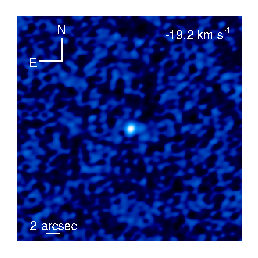
\includegraphics[trim=45pt 0pt 30pt 0pt, width=8.0cm, height=6.8cm]{f2.eps}
\caption{Integrated intensity image of the D configuration channel maps that contain the discrete second source approximately 5$\arcsec$ S-W of $\alpha$ Ori. Contours for the integrated intensity are 1$\sigma$, 1.5$\sigma$, 2$\sigma$, and 3$\sigma$ (1$\sigma$ = 1.3 Jy beam${}^{-1}$ km s${}^{-1}$). The size of the restoring beam is shown in white in the bottom left corner.}
\label{fig:fig2}
\end{figure}

\clearpage

\begin{figure}[hbt!]
%\centering
\mbox{
          \includegraphics[]{chan41.ps}
          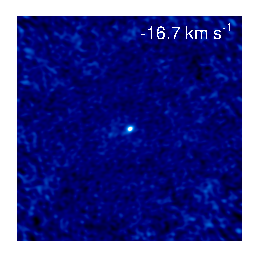
\includegraphics[]{chan40.ps}
          }
\\
\mbox{
          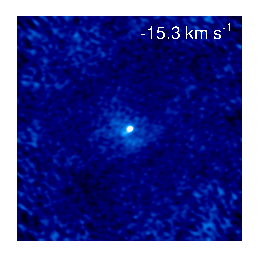
\includegraphics[]{chan39.ps}
          \includegraphics[]{chan38.ps}
          }
\\
\mbox{
          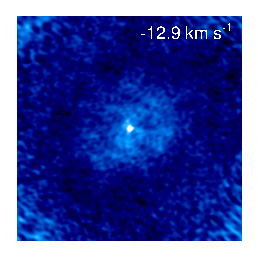
\includegraphics[]{chan37.ps}
          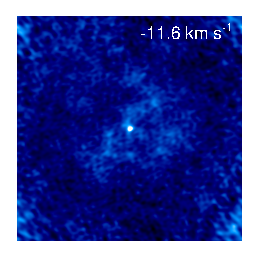
\includegraphics[]{chan36.ps}
         }
\\
\mbox{
          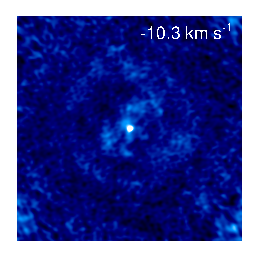
\includegraphics[]{chan35.ps}
          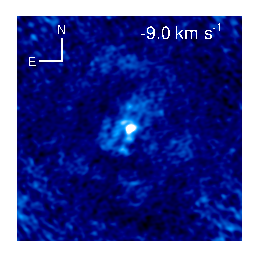
\includegraphics[]{chan34.ps}
         }
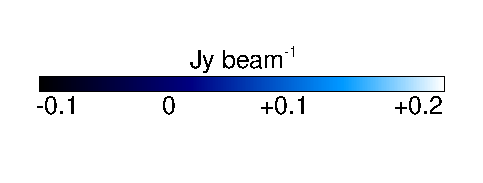
\includegraphics[trim=0pt 20pt 180pt 10pt]{color_bar.ps}
\caption{8 channel maps from the combined configuration image cube. The peak emission has been cut at 0.2 Jy beam${{}^{-1}}$ to emphasize the fainter emission. The color scale is linear and has been normalized to this maximum cutoff and minimum value of each channel. The emission at the corners of each map is a result of the primary beam correction.}
\label{fig:fig3}
\end{figure}


\clearpage

\begin{figure}
\epsscale{1.2}
\plotone{f13.eps}
\caption{Spectral profiles of the low spectral resolution combined image cube for circular extraction areas of radius 1$\arcsec$, 2$\arcsec$, 4$\arcsec$, 6$\arcsec$, 8$\arcsec$, and 10$\arcsec$.}
\label{fig:fig4}
\end{figure}

\clearpage

\begin{figure}
\epsscale{1.2}
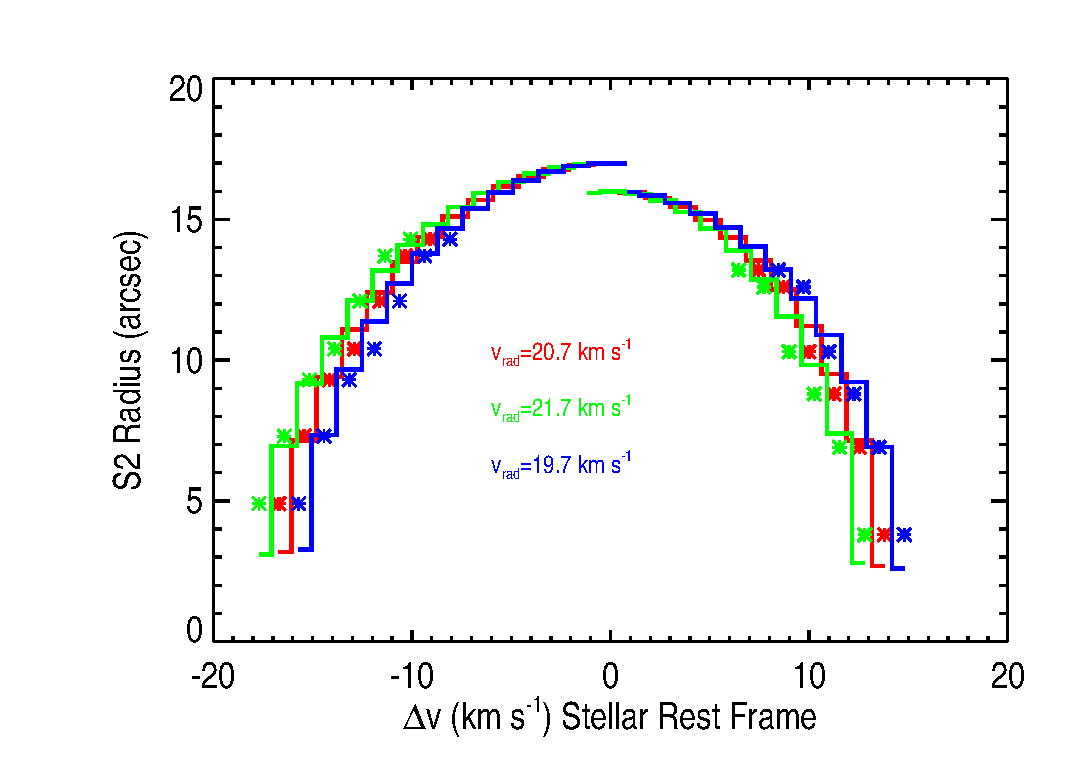
\includegraphics[trim=45pt 0pt 30pt 0pt, width=7.5cm, height=6.5cm]{s2_size.eps}
\caption{The derived shell radius as a function of velocity (blue points) overplotted with two model shells. The green line corresponds to a shell with a maximum size of 17$\arcsec$ and an outflow velocity of 17 km s${}^{-1}$ while the red line corresponds to a shell with a maximum size of 16$\arcsec$ and an outflow velocity of 14 km s${}^{-1}$.}
\label{fig:fig4}
\end{figure}

\clearpage

\begin{figure}
\epsscale{1.0}
\includegraphics[angle=90, trim=5pt 0pt 0pt 0pt,width=7.5cm, height=7.5cm]{aori_mcdonald.ps}
\caption{The .}
\label{fig:fig5}
\end{figure}

\clearpage

\begin{deluxetable}{ccccccc}
\tabletypesize{\scriptsize}
\tablecaption{CARMA Observations}
\tablewidth{0pt}
\tablehead{
\colhead{Observation} & \colhead{Configuration} & \colhead{Time on Source} & \colhead{Flux} 	& \colhead{Phase} & \colhead{Image Cube\tablenotemark{a}}\\
\colhead{Date}  	      & 		   	  & \colhead{(hr)} 		  & \colhead{Calibrator} & \colhead{Calibrators} & \colhead{Dynamic Range\tablenotemark{b}}}
}
\startdata
2007 Jun 18 & D & 0.9 & 0530+135 & 0530+135, 0532+075 &  13.01 \\
2007 Jun 21 & D & 3.0 & 0530+135 & 0530+135, 0532+075 &  12.98 \\
2007 Jun 24 & D & 2.1 & 0530+135 & 0530+135, 0532+075 &  13.75 \\
2007 Jun 25 & D & 2.4 & 0530+135 & 0530+135, 0532+075 &  15.66 \\
2009 Jul 07 & E & 3.2 & 3C120 & 3C120, 0532+075 & 15.04 \\
2009 Nov 05 & C & 1.2 & 3C120 & 3C120, 0532+075 & 10.94 \\
2009 Nov 09 & C & 3.0 & 3C120 & 3C120, 0532+075 & 16.81 \\
2009 Nov 15 & C & 1.0 & 3C120 & 3C120, 0532+075 & 11.35 \\
2009 Nov 16 & C & 3.2 & 3C120 & 3C120, 0532+075 & 18.47  \\
All & C & 8.4 & \nodata & \nodata &   29.28 \\
All & D & 9.5 & \nodata & \nodata &   22.38 \\
All & Combined & 21.2 & \nodata & \nodata &   31.72 \\
\enddata
\tablenotetext{a}{Channel width of 1.3 km s$\rm{{}^{-1}}$ and not corrected for primary beam attenuation.}
\tablenotetext{b}{The peak emmision of the image cube divided by the root mean square of the residual image.}
\label{tab:tab1}
\end{deluxetable}

\clearpage

\begin{deluxetable}{cccc}
\tabletypesize{\scriptsize}
\tablecaption{CARMA Continuum Fluxes}
\tablewidth{0pt}
\tablehead{
\colhead{Configuration} & \colhead{Restoring Beam } & \colhead{Flux} & \colhead{Uncertainty } \\
	      & ($\arcsec \times \arcsec$)   	  & \colhead{(mJy)}    & \colhead{(mJy)} 
}
\startdata
C & 0.96 \times 0.76 & 234 & 18\\
D & 2.33 \times 1.87 & 389 & 72\\
E & 4.93 \times 3.84 & 278 & 40 \\
Combined & 1.05 \times 0.84 & 289 & 21 \\
\enddata
\label{tab:tab2}
\end{deluxetable}
\end{document}